% !TeX program = lualatex
% ================================================================
% Polish Parallel Text Version of CirclesIntroductoryStarters
%
% Generated by the server using the following settings:
%
%   language            Polish (pol)
%   text direction      left to right
%   font                Noto Serif
%   fallback font       Noto Serif
%   built from          latex/starters/targeted/KS3/circles/circlesIntroductoryStarters.tex
%   vocabulary key      latex/starters/targeted/KS3/circles/circlesIntroductoryStarters/L2/pol/circlesIntroductoryStarters_polishKey.tex
%   tier 3 vocabulary   green   RGB 0 128 0
%   English text        black   RGB 0 0 0
%   Polish text         purple  RGB 112 48 160
%   layout macros       version 2
%
% Please don't edit any information in this comment block - the server
% compares it against the current settings and rebuilds this file when
% they differ, so changes here would be overwritten. However, feel free
% to make updates to the LaTeX below if you want to edit it.
% ================================================================

\documentclass{beamer}
\usepackage{tikz}
\usetikzlibrary{calc,arrows.meta,patterns}
\usepackage{multicol}
\usepackage{amsmath}
\usetikzlibrary{overlay-beamer-styles}
% Characters this language's font has not got are borrowed from another,
% rather than being silently dropped - see docs/translated-sheet-latex.md
\directlua{%
  if luaotfload and luaotfload.add_fallback then
    luaotfload.add_fallback("eallatinfallback",
      { "Noto Serif:mode=harf;" })
  else
    tex.error("this luaotfload is too old to register a fallback font")
  end
}
\usepackage[english]{babel}
\babelprovide[import]{polish}
\babelfont[polish]{rm}[Renderer=Harfbuzz, BoldFont={Noto Serif}, ItalicFont={Noto Serif}, BoldItalicFont={Noto Serif}, RawFeature={fallback=eallatinfallback}]{Noto Serif}
\babelfont[polish]{sf}[Renderer=Harfbuzz, BoldFont={Noto Serif}, ItalicFont={Noto Serif}, BoldItalicFont={Noto Serif}, RawFeature={fallback=eallatinfallback}]{Noto Serif}
\newcommand{\ealtext}[1]{\foreignlanguage{polish}{#1}}
\newcommand{\ealtextblock}[1]{{\raggedright\foreignlanguage{polish}{#1}\par}}
% ================================================================
% EAL layout helpers
% ================================================================
\usepackage{xcolor}

\definecolor{ealkeycolour}{RGB}{0,128,0}
\definecolor{ealenglish}{RGB}{0,0,0}
\definecolor{ealtwocolour}{RGB}{112,48,160}

\newsavebox{\ealboxen}
\newsavebox{\ealboxtr}
\newlength{\ealglosswd}
\newlength{\ealglossraise}
\setlength{\ealglossraise}{1.15em}

% a tier 3 word, in English and in translation alike
\newcommand{\ealkey}[1]{\textcolor{ealkeycolour}{#1}}
\newcommand{\ealkeytr}[1]{\textcolor{ealkeycolour}{\ealtext{#1}}}

% One translated word above one English word. Built from kernel
% primitives, never a tabular, which would break wherever the sheet
% loads array, booktabs or tabularx. The box is as wide as the wider of
% the two, so a long translation pushes its neighbours aside instead of
% overlapping them, and it claims its full height so a table row or a
% TikZ node makes room for it.
\newcommand{\ealgloss}[2]{%
  \sbox{\ealboxen}{\ealkey{#1}}%
  \sbox{\ealboxtr}{\small\textcolor{ealtwocolour}{\ealtext{#2}}}%
  \setlength{\ealglosswd}{\wd\ealboxen}%
  \ifdim\wd\ealboxtr>\ealglosswd\setlength{\ealglosswd}{\wd\ealboxtr}\fi
  \leavevmode
  \makebox[\ealglosswd][c]{%
    \makebox[0pt][c]{\usebox{\ealboxen}}%
    \makebox[0pt][c]{\raisebox{\ealglossraise}{\usebox{\ealboxtr}}}%
  }%
}

% opens up line spacing around a block of glosses, so the raised
% translations sit clear of the line above
\newenvironment{ealglossed}{\par\linespread{2.1}\selectfont\ignorespaces}{\par}

% a whole translated sentence above its English counterpart. block level,
% so it does not belong inside a tabular cell
\newcommand{\ealpara}[2]{%
  \par\addvspace{0.5\baselineskip}%
  {\color{ealtwocolour}\ealtextblock{#1}}%
  \penalty200
  {\color{ealenglish}#2\par}%
  \addvspace{0.5\baselineskip}%
}

\begin{document}

\frame{\titlepage}

%------------------------------------------------
% SLIDE 1: Arithmetic, Lengths & Decimals (No Circles)
%------------------------------------------------
\begin{frame}{Starter}

\begin{columns}

\column{0.3\textwidth}
\begin{center}
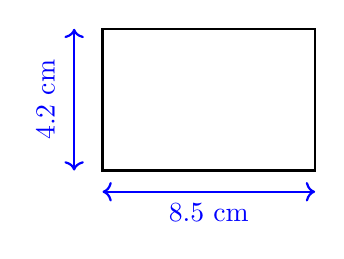
\begin{tikzpicture}[scale=0.9]
  % Rectangle for perimeter
  \draw[thick] (0,0) rectangle (3,2);
  \draw[blue, thick, <->] (0,-0.3) -- (3,-0.3);
  \node[blue] at (1.5,-0.6) {$8.5$ cm};
  \draw[blue, thick, <->] (-0.4,0) -- (-0.4,2);
  \node[blue, rotate=90] at (-0.8,1) {$4.2$ cm};
  
\end{tikzpicture}
\end{center}

\column{0.7\textwidth}
\small
\begin{enumerate}
    \begin{multicols}{2}
        \item $13 + 9 = \ashowq{22}$
        \item $5.8 - 1.9 = \ashowq{3.9}$
    \end{multicols}
    \begin{multicols}{2}
        \item $6 \times 8 = \ashowq{48}$
        \item $4 \times 3.5 \ \ashowq{14}$
  \end{multicols}
  \item \ealpara{\ealkeytr{Zaokrąglij} $3.14159$ do 2 \ealkeytr{miejsc dziesiętnych}.}{Round $3.14159$ to 2 \ealkey{decimal places}. \ashow{3.14}}
  \item \ealpara{Ołówek ma długość $12.8$ cm. Ile to milimetrów?}{A pencil is $12.8$ cm long. How many millimetres is this? \ablank{128 mm}}
\end{enumerate}

\begin{enumerate}
  \setcounter{enumi}{4}
  \item \ealpara{Znajdź \ealkeytr{obwód} pokazanego prostokąta.}{Find the \ealkey{perimeter} of the rectangle shown. \ashow{25.4 cm}}
  \item \ealpara{\ealkeytr{Obwód} kwadratu wynosi $26$ cm. Jaka jest długość jednego boku?}{The \ealkey{perimeter} of a square is $26$ cm. What is the length of one side? \ashow{6.5 cm}}
  \item \ealpara{\ealkeytr{Obwód} trójkąta \ealkeytr{równobocznego} wynosi $12.9$ cm. Znajdź długość jednego boku, a następnie \ealkeytr{obwód} \ealkeytr{sześciokąta} \ealkeytr{foremnego} o tej samej długości boku. \ashow{$4.3$ cm; \ealkeytr{sześciokąt}: $25.8$ cm}}{The \ealkey{perimeter} of an \ealkey{equilateral} triangle is $12.9$ cm. 
    Find the length of one side, and then the \ealkey{perimeter} of a \ealkey{regular} \ealkey{hexagon} with the same side length. \ashow{$4.3$ cm; \ealkey{hexagon}: $25.8$ cm}}
\end{enumerate}

\end{columns}
\end{frame}

%------------------------------------------------
% SLIDE 2: Arithmetic + Radius, Diameter, Chord
%------------------------------------------------
\begin{frame}{Starter}
\vspace{-2em}
\begin{columns}

\column{0.3\textwidth}
\begin{center}
\begin{tikzpicture}[scale=0.75]
  % Circle
  \draw[thick] (0,0) circle (2cm);

  % Center
  \fill (0,0) circle (0.05);
  \node[below left] at (0,0) {$O$};

  % Radius
  \draw[red, thick] (0,0) -- (1.2,1.6);

  % Diameter
  \draw[blue, thick] (-2,0) -- (2,0);

  % Chord (not through center)
  \draw[thick] (-1.5,-1.323) -- (1.2,-1.6);

  % --- Q5 answer: name the lines on the diagram ---
  \node[anslab, above] at (-0.85,0.05) {diameter};
  \node[anslab, above, rotate=-6] at (-0.15,-1.46) {chord};
\end{tikzpicture}
\end{center}

\column{0.7\textwidth}
\small
\begin{enumerate}
\begin{multicols}{2}
  \item $24 \div 6$ \ashow{$=4$}
  \item $72 \div 8$ \ashow{$=9$}
  \end{multicols}
  \begin{multicols}{2}
  \item \ealpara{Podwój $15.5$.}{Double $15.5$ \ashow{$=31$}}
  \item \ealpara{Podziel $31.4$ na pół.}{Halve $31.4$ \ashow{$=15.7$}}
  \end{multicols}
  \item \ealpara{Ile centymetrów ma $1.2$ metra?}{How many centimetres in $1.2$ metres? \ashow{120 cm}}
  \item \ealpara{Prawda czy fałsz? $2.5 \times 4 = 10$ \ashow{Prawda}}{True or false? $2.5 \times 4 = 10$ \ashow{True}}
\end{enumerate}

\begin{enumerate}
  \setcounter{enumi}{4}
  \item \ealpara{Na diagramie, która linia to \textbf{\ealkeytr{średnica}}? Czym różni się od \ealkeytr{cięciwy}? \ashow{\ealkeytr{Średnica} przechodzi przez środek.}}{On the diagram, which line is the \textbf{\ealkey{diameter}}? 
    How is it different from a \ealkey{chord}? \ashow{A \ealkey{diameter} passes through the centre.}}
  \item \ealpara{Jeśli \ealkeytr{promień} okręgu wynosi $7$ cm, ile wynosi jego \ealkeytr{średnica}?}{If the \ealkey{radius} of a circle is $7$ cm, what is its \ealkey{diameter}? \ashow{14 cm}}
  \item \ealpara{\ealkeytr{Średnica} okręgu wynosi $18$ mm. Znajdź jego \ealkeytr{promień}.}{The \ealkey{diameter} of a circle is $18$ mm. Find its \ealkey{radius}. \ablank{9 mm}}
  \item \ealpara{\ealkeytr{Cięciwa} o długości $8$ cm jest narysowana wewnątrz okręgu o \ealkeytr{promieniu} $5$ cm. Czy ta \ealkeytr{cięciwa} jest \ealkeytr{średnicą}? Dlaczego tak, a dlaczego nie? \ashow{Nie; \ealkeytr{średnica} miałaby $10$ cm.}}{A \ealkey{chord} of length $8$ cm is drawn inside a circle of \ealkey{radius} $5$ cm.
    Is the \ealkey{chord} a \ealkey{diameter}? Why, or why not?. \ashow{No; a \ealkey{diameter} would be $10$ cm.}}
\end{enumerate}

\end{columns}
\end{frame}

%------------------------------------------------
% SLIDE 3: Arithmetic + Segments, Sectors, Arcs, Tangents
%------------------------------------------------
\begin{frame}{Starter}

\vspace{-2em}

\begin{columns}

\column{0.35\textwidth}

\begin{center}
\begin{tikzpicture}[scale=0.75]
  % Circle
  \draw[thick] (0,0) circle (2cm);
  \fill (0,0) circle (0.05);
  \node[below] at (0,-0.1) {$O$};

  % --- Q6 answers: drawn on the circle ---
  % Sector
  \fill[ansfill] (0,0) -- (105:2) arc (105:165:2) -- cycle;
  \draw[ans] (0,0) -- (105:2);
  \draw[ans] (0,0) -- (165:2);
  \node[anslab] at (135:1.2) {sector};

  % Arc
  \draw[ans, ultra thick] (25:2) arc (25:75:2);
  \node[anslab] at (50:1.5) {arc};

  % Tangent
  \draw[ans] (-2,-1.2) -- (-2,1.2);
  \node[anslab, rotate=90] at (-2.22,0) {tangent};

  % Segment
  \fill[ansfill] (-75:2) arc (-75:-5:2) -- cycle;
  \draw[ans] (-75:2) -- (-5:2);
  \draw[ans, -{Stealth[length=1.5mm]}] (0.95,-2.45) -- (1.42,-1.25);
  \node[anslab] at (0.95,-2.65) {segment};
\end{tikzpicture}

\vspace{3em}

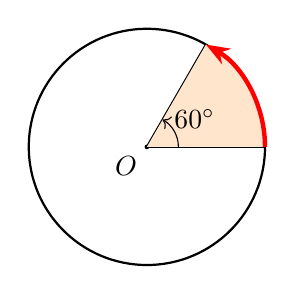
\begin{tikzpicture}[scale=1]
  % Circle
  \draw[thick] (0,0) circle (1.5cm);
  
  % Centre
  \fill (0,0) circle (0.03);
  \node[below left] at (0,0) {$O$};
  
  % Radii that bound the 60° sector
  \draw[thick] (0,0) -- (0:1.5);          % right horizontal radius
  \draw[thick] (0,0) -- (60:1.5);         % radius at 60°
  

  
  % Optional: shade the sector lightly
  \fill[orange!20] (0,0) -- (0:1.5) arc (0:60:1.5) -- cycle;

    % Highlight the arc (thick, coloured, with arrow)
  \draw[red, ultra thick, -{Stealth[length=3mm]}] 
    (0:1.5) arc (0:60:1.5);
  
  % Angle arc and label
  \draw[->] (0.4,0) arc (0:60:0.4);
  \node at (30:0.7) {$60^\circ$};
  
\end{tikzpicture}

\end{center}


\column{0.65\textwidth}
\small
\begin{enumerate}
\begin{multicols}{2}
  \item $3.2 \times 5$ \ashow{$=16$}
  \item $1.8 \times 4$ \ashow{$=7.2$}
  \end{multicols}
  \begin{multicols}{2}
    \item  $45 \div 10$ \ashow{$=4.5$}
    \item $90 \div 100$ \ashow{$=0.9$}
  \end{multicols}
  \item \ealpara{Ile wynosi $\frac{1}{4}$ z $360^\circ$?}{What is $\frac{1}{4}$ of $360^\circ$? \ashow{$90^\circ$}}
\end{enumerate}

\begin{enumerate}
  \setcounter{enumi}{5}
  \item \ealpara{Przerysuj diagram i narysuj z podpisami:}{Copy the diagram, and draw with labels:}
    \begin{multicols}{2}
    \begin{itemize}
      \item \ealpara{\ealkeytr{Wycinek koła}}{A \ealkey{sector}}
      \item \ealpara{\ealkeytr{Łuk}}{An \ealkey{arc}}
      \item \ealpara{\ealkeytr{Styczna}}{A \ealkey{tangent}}
      \item \ealpara{\ealkeytr{Odcinek koła}}{A \ealkey{segment}}
    \end{itemize}
    \end{multicols}
  \item \ealpara{Jeśli \ealkeytr{promień} wynosi $6$ cm, ile wynosi cały \ealkeytr{obwód}? (Użyj $\pi \approx 3.14$)}{If the \ealkey{radius} is $6$ cm, what is the whole \ealkey{circumference}? (Use $\pi \approx 3.14$) \ashow{$37.68$ cm}}
  \item \ealpara{Dla pokazanego \ealkeytr{wycinka koła}, jakim \ealkeytr{ułamkiem} \ealkeytr{obwodu} jest długość \ealkeytr{łuku}? Oblicz długość \ealkeytr{łuku}, jeśli cały okrąg ma \ealkeytr{obwód} 24cm.}{For the \ealkey{sector} shown, what \ealkey{fraction} of the \ealkey{circumference} is the \ealkey{arc} length? Calculate the \ealkey{arc} length if the whole circle has a \ealkey{circumference} of 24cm. \ashow{$\frac{1}{6}$; $4$ cm}}

\end{enumerate}

\end{columns}
\end{frame}

%------------------------------------------------
% SLIDE 4: Arithmetic + Labelling, Pi, Diameter
%------------------------------------------------
\begin{frame}{Starter}

\vspace{-2em}

\begin{columns}

\column{0.3\textwidth}
\begin{center}
\begin{tikzpicture}[scale=0.75]
  % Circle with labels
  \draw[thick] (0,0) circle (2cm);
  \fill (0,0) circle (0.05);

  \draw[blue, thick] (-2,0) -- (2,0);

  \draw[red, thick] (0,0) -- (40:2);

  % --- Q8 answer: label the parts on the diagram ---
  \node[anslab, below right, inner sep=2pt] at (0,0) {centre};
  \node[anslab, above, rotate=40] at (40:1.1) {radius};
  \node[anslab, above] at (-1,0.02) {diameter};
  \draw[ans, -{Stealth[length=1.5mm]}] (0,2.5) -- (100:2.05);
  \node[anslab, above] at (0,2.5) {circumference};

  % --- Q9 answer: a chord shorter than the radius ---
  \draw[ans] (190:2) -- (240:2);
  \node[anslab] at (215:1.3) {$<r$};

  % --- Q10 answer: a chord longer than the radius ---
  \draw[ans] (-80:2) -- (10:2);
  \node[anslab] at (-33:1.15) {$>r$};
\end{tikzpicture}

\end{center}

\column{0.7\textwidth}
\small
\begin{enumerate}
\begin{multicols}{2}
  \item $12 \times 3 $ \ashow{$=36$}
  \item $4 \times 3.14$ \ashow{$=12.56$}
\end{multicols}
\begin{multicols}{2}
  \item $6.28 \div 2 $ \ashow{$=3.14$} 
  \item $ 9.42 \div 3$ \ashow{$=3.14$}
  \end{multicols}
  \item \ealpara{\ealkeytr{Zaokrąglij} $3.14159265$ do 3 \ealkeytr{miejsc dziesiętnych}.}{Round $3.14159265$ to 3 \ealkey{decimal places}. \ashow{3.142}}
  \begin{multicols}{2}
  \item \ealpara{Podwój $3.14$.}{Double $3.14$ \ashow{$=6.28$}}
  \item \ealpara{Podziel $12.56$ na pół.}{halve $12.56$ \ashow{$=6.28$}}
  \end{multicols}
\end{enumerate}
\vspace{-0.5em}
\begin{enumerate}
  \setcounter{enumi}{7}
  \item \ealpara{Przerysuj i podpisz na diagramie: środek, \ealkeytr{promień}, \ealkeytr{średnica}, \ealkeytr{obwód}.}{Copy and label on the diagram: 
    centre, \ealkey{radius}, \ealkey{diameter}, \ealkey{circumference}.}
    \item \ealpara{Narysuj na diagramie \ealkeytr{cięciwę} krótszą niż \ealkeytr{promień}.}{Draw a \ealkey{chord} on the diagram shorter than the \ealkey{radius}}
    \item \ealpara{Narysuj na diagramie \ealkeytr{cięciwę} dłuższą niż \ealkeytr{promień}.}{Draw a \ealkey{chord} on the diagram longer than the \ealkey{radius}}
  
  \item \ealpara{Jeśli \ealkeytr{średnica} wynosi $8$ cm, ile wynosi:}{If the \ealkey{diameter} is $8$ cm, what is:}
    \begin{itemize}
      \item \ealpara{\ealkeytr{promień}?}{the \ealkey{radius}? \ashow{$4$ cm}}
      \item \ealpara{\ealkeytr{obwód}? ($\pi \approx 3.14$)}{the \ealkey{circumference}? ($\pi \approx 3.14$) \ashow{$25.12$ cm}}
    \end{itemize}
 
\end{enumerate}

\end{columns}
\end{frame}

\end{document}